
\documentclass[9pt,a4paper]{extarticle}

\usepackage[margin=1.7cm]{geometry}
\usepackage[T1]{fontenc}
\usepackage{lmodern}
\usepackage{microtype}
\usepackage{graphicx}
\usepackage{booktabs}
\usepackage{amsmath}
\usepackage{xcolor}
\usepackage{url}
\usepackage[font=small,labelfont=bf]{caption}

\setlength{\parindent}{0pt}
\setlength{\parskip}{4pt}

\newcommand{\code}[1]{\texttt{#1}}

\title{\textbf{Comparing Apache Spark, Dask, and RAPIDS}\\
on Batch and Iterative Workloads}
\author{}
\date{}

\begin{document}
\maketitle
\begin{figure*}[t]
\centering
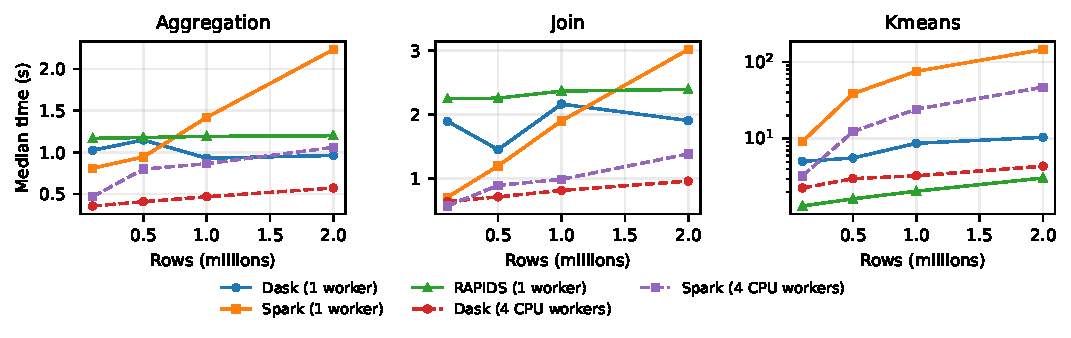
\includegraphics[width=.88\textwidth]{runtime.pdf}
\caption{Median runtime versus dataset size. Solid: one worker; dashed: four CPU workers. K-means uses a logarithmic vertical axis.}
\label{fig:runtime}
\end{figure*}
\section{Objective and implementation}
We implemented comparable data-processing pipelines in \textbf{Apache Spark} (DataFrame API), \textbf{Dask} (CPU DataFrames), and \textbf{RAPIDS/Dask-cuDF} (GPU DataFrames). The objective was to evaluate how execution model and workload characteristics affect end-to-end runtime, CPU parallel scaling, and memory use. The submission includes implementations, data preparation, benchmark runners, validation, CSV results, and plotting scripts.

\section{Dataset and workloads}
We used public \textbf{NYC TLC Yellow Taxi} trip records from January--March 2024, stored as Parquet, together with the taxi-zone lookup CSV. The original monthly files are available at \url{https://www.nyc.gov/site/tlc/about/tlc-trip-record-data.page}. A shared preparation script creates four subsets containing \textbf{100K, 500K, 1M, and 2M} trips; these prepared files are omitted from the submission because of their size.

All frameworks implement three workloads: (1) \textbf{aggregation}, grouping by pickup zone and hour to compute counts and fare/distance statistics; (2) \textbf{join}, enriching trips with zone information and joining derived zone statistics; and (3) \textbf{K-means}, running ten Lloyd iterations with five centroids and fixed initialization on selected numeric trip features. The same prepared input files are used across frameworks.

\section{Experimental methodology}
Dask and Spark were tested with \textbf{1, 2, 4, and 8 CPU workers}, using 16 partitions; RAPIDS ran on a \textbf{single NVIDIA Tesla T4} with 16 partitions. Each workload/size/configuration had \textbf{one untimed warmup and three timed repetitions}. We report the median wall-clock time; 144 Dask, 144 Spark, and 36 RAPIDS measurements completed successfully (324 total). CPU experiments used Python 3.14.8; Spark used Java 17. RAPIDS used Python 3.13.16, cuDF 26.06, and a Tesla T4 (15 GiB). Exact CPU processor/RAM details were not captured in the supplied configuration records.

The runners recorded process resident memory (RSS); RAPIDS additionally sampled GPU device memory. These are different metrics and are \emph{not} directly interchangeable. We compared output row counts and checksums across frameworks: all recorded configurations agreed within floating-point tolerance. Checksums are useful sanity checks but do not establish complete equivalence of intermediate execution plans.



\section{Results}
Figure 1 shows that aggregation and join times change relatively little with increasing dataset size, especially for RAPIDS; fixed execution and scheduling costs are plausible contributors at these scales. K-means grows more markedly and shows the strongest benefit from GPU execution. At 2M rows, the medians in Table 1 show that \textbf{single-worker Dask beats RAPIDS on aggregation and join}, whereas \textbf{RAPIDS is 3.40$\times$ faster than single-worker Dask and 47.49$\times$ faster than single-worker Spark on K-means}. These ratios compare observed systems, not equivalent CPU/GPU hardware budgets.

\begin{table}[h]
\centering\caption{Median seconds at 2M rows (lower is better).}
\small\setlength{\tabcolsep}{4pt}
\begin{tabular}{lrrr}\toprule
Workload & Dask (1) & Spark (1) & RAPIDS (1 GPU)\\\midrule
Aggregation & \textbf{0.964} & 2.234 & 1.200\\
Join & \textbf{1.909} & 3.018 & 2.396\\
K-means & 10.403 & 145.320 & \textbf{3.060}\\\bottomrule
\end{tabular}
\end{table}

\begin{figure}[h]
\centering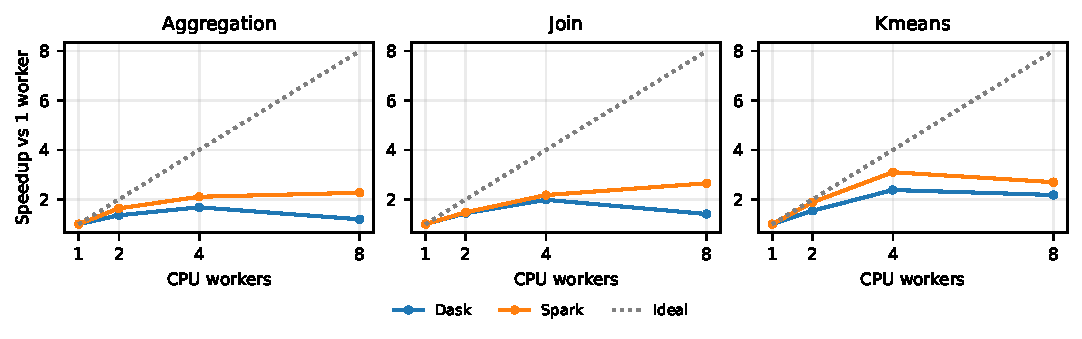
\includegraphics[width=\columnwidth]{scaling.pdf}
\caption{CPU speedup at 2M rows relative to each framework's one-worker runtime. The dotted line represents ideal linear scaling. RAPIDS is excluded because only one GPU was available.}
\end{figure}

Figure 2 illustrates diminishing CPU scaling returns. For example, Dask K-means improves from 10.40 s with one worker to 4.37 s with four, then slows to 4.78 s with eight. Spark K-means improves from 145.32 s to 46.91 s at four workers, but rises to 53.90 s at eight. Scheduling, synchronization, and data movement are possible causes; the experiments did not separately profile these costs. GPU memory sampling and CPU RSS also reflect caching and allocator behavior, so memory deltas should not be treated as exact per-operation allocation sizes.

\section{Limitations and conclusions}
The GPU and CPU runs used \textbf{different machines and software environments}; thus performance ratios are not hardware-normalized acceleration factors. Three repetitions permit descriptive variability analysis but limited statistical inference. The join checksum could be insensitive to some intermediate join operations, and K-means centroid sums do not prove identical cluster assignments. Finally, no direct shuffle-byte or GPU-utilization trace was retained.

Overall, \textbf{no framework wins every workload}: CPU Dask is competitive for relatively lightweight batch operations, while RAPIDS provides a substantial observed advantage for iterative K-means at the largest tested size. The results suggest choosing an execution engine based on workload and overhead rather than GPU availability alone.

\section{Reproducing the experiments}
From the repository root, download the three 2024 Yellow Taxi Parquet files into \code{data/raw/} and run \code{python common/prepare\_data.py --months 2024-01 2024-02 2024-03 --sizes 100000 500000 1000000 2000000}. Install the CPU requirements in separate environments (\code{requirements.txt} for Dask; \code{requirements-spark.txt} and Java 17 for Spark), then run \code{bash run\_dask\_final.sh} and \code{bash run\_spark\_final.sh}. On a CUDA-enabled machine with compatible RAPIDS/cuDF installed, run \code{bash run\_rapids\_smoke.sh} followed by \code{bash run\_rapids\_final.sh}. Outputs are stored under \code{results/}; analysis scripts are in \code{analysis/}. The README documents environment setup and file locations.
\end{document}
